\chapter{Mask}


\section{Boolean operations}

After segmenting, some boolean operations can be performed between masks. The boolean operations supported by InVesalius are:

\begin{itemize}
	\item \textbf{Union}, perform union between two masks;
	\item \textbf{Difference}, perform difference from the first mask to the second one;
	\item \textbf{Intersection}, keeps what is common in both masks.
	\item \textbf{Exclusive disjunction (XOR)}: keeps the regions of the first mask which are not in the second mask and regions from the second mask which are no in the first mask.
\end{itemize}

To use this tool go to the \textbf{Tools}, menu, select \textbf{Mask}, and then Boolean operations as shown in Figure~\ref{fig:booleano_menu}. Select the first mask, the operation to be performed and the second mask as shown in Figure~\ref{fig:booleano_janela} then click \textbf{OK}.


\begin{figure}[!htb]
\centering
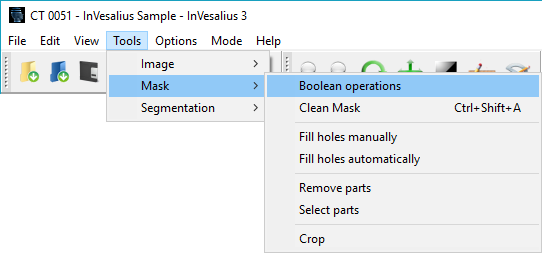
\includegraphics[scale=0.5]{mask_operation_boolean_menu_en.png}
\caption{Menu to open boolean operations tool.}
\label{fig:booleano_menu}
\end{figure}


\begin{figure}[!htb]
\centering
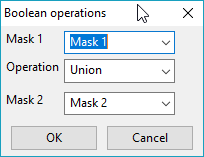
\includegraphics[scale=0.5]{mask_boolean_dialog_en.png}
\caption{Boolean operations tool.}
\label{fig:booleano_janela}
\end{figure}

Figure~\ref{fig:op_boolana} shows some examples of utilization of boolean operations tool.

\begin{figure}[!htb]
  \centering
  \subfloat[Mask A]{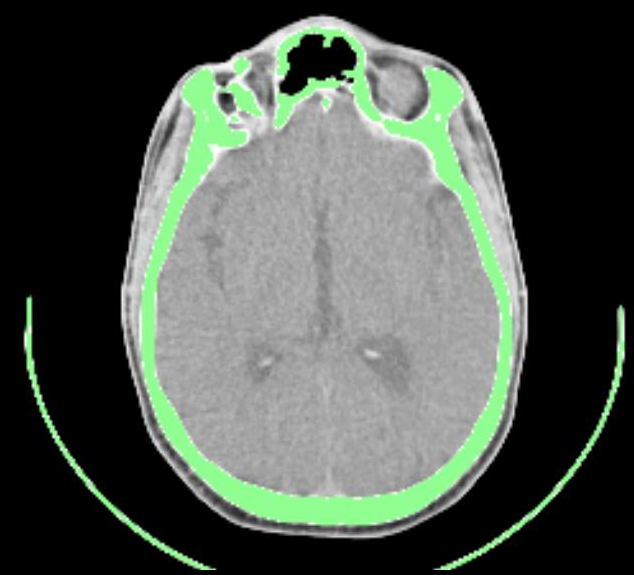
\includegraphics[width=0.332\textwidth]{booleano_m_a.png}}
  \hfill
  \subfloat[Mask B]{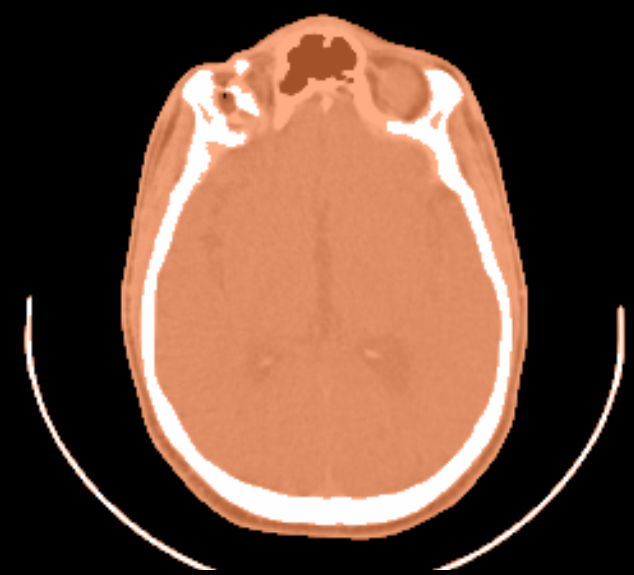
\includegraphics[width=0.332\textwidth]{booleano_m_b.png}}
  \hfill
  \subfloat[Union (A $\cup$ B)]{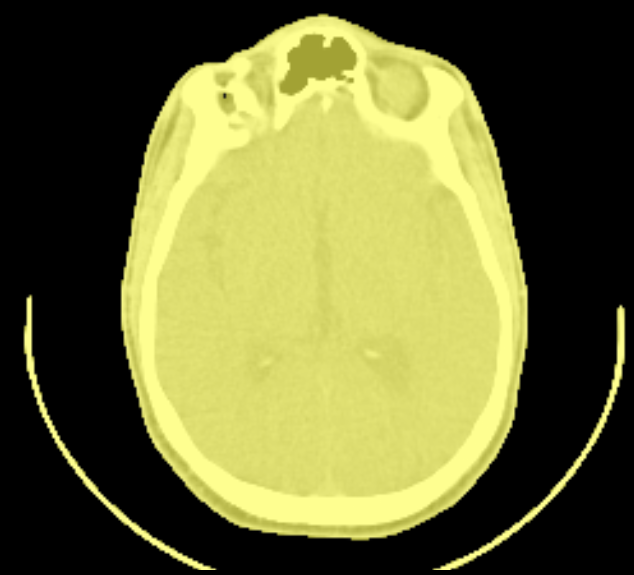
\includegraphics[width=0.332\textwidth]{booleano_uniao.png}}
  \hfill
  \subfloat[Difference (A - B)]{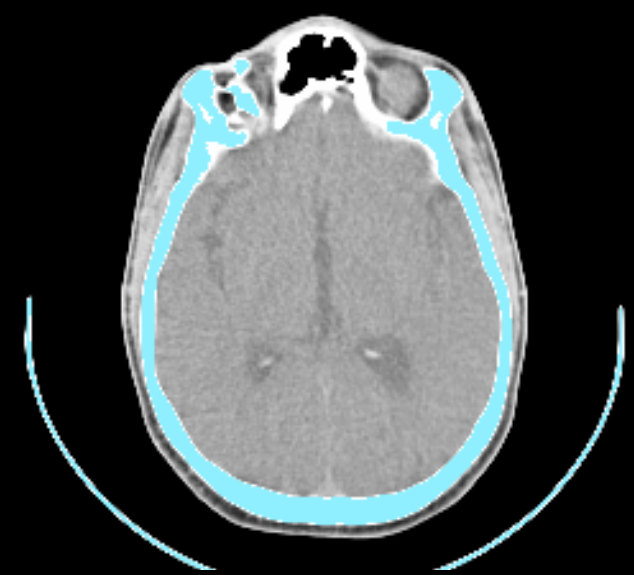
\includegraphics[width=0.332\textwidth]{booleano_dif.png}}
  \hfill
  \subfloat[Intersection (A $\cap$ B)]{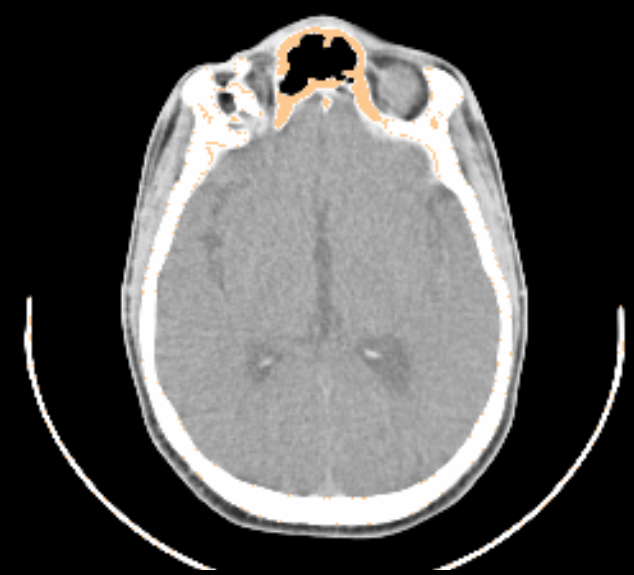
\includegraphics[width=0.332\textwidth]{booleano_interc.png}}
  \hfill
  \subfloat[Exclusive disjunction (A $\oplus$ B)]{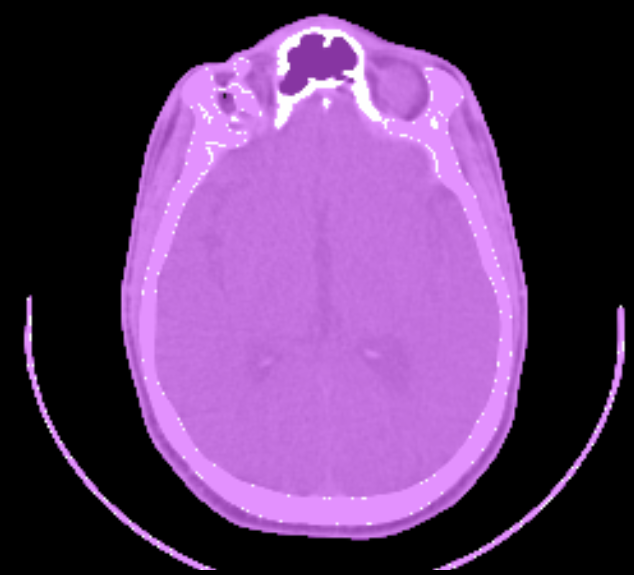
\includegraphics[width=0.332\textwidth]{booleano_disj_exc.png}}
  \caption{example of boolean operations.}
  \label{fig:op_boolana}
\end{figure}

\section{Mask cleaning}
\label{cap:limpeza_mascara}

A mask can be cleaned, as shown in Figure~\ref{fig:limpeza_mascara}. This is recommended before inserting Watershed markers. This tool is located on the \textbf{Tools} menu. Select \textbf{Mask}, then \textbf{Clean mask}, or use the shortcut \textbf{CTRL+SHIFT+A}.

\begin{figure}[!htb]
\centering
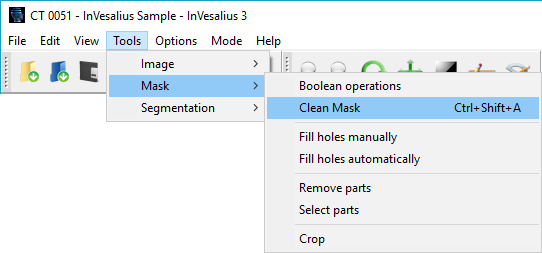
\includegraphics[scale=0.5]{mask_clean_menu_en.png}
\caption{Mask cleaning}
\label{fig:limpeza_mascara}
\end{figure}

\section{Fill holes manually}

Segmentation may leave some unwanted holes. It's recommended to fill them because the surface generated from this mask may have some inconsistencies. To do this access the menu \textbf{Tools}, \textbf{Mask}, \textbf{Fill holes manually} (figure~\ref{fig:menu_mask_manual_fill_holes}). A dialog window will be shown (figure~\ref{fig:mask_manual_fill_holes_window}) to configure the parameters.

\begin{figure}[!htb]
\centering
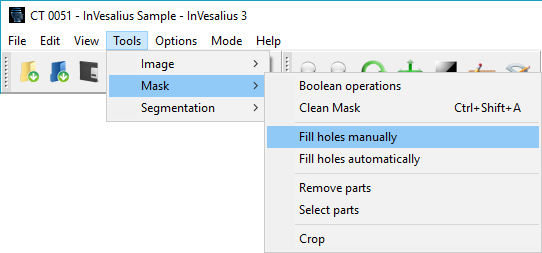
\includegraphics[scale=0.4]{menu_mask_manual_fill_holes_en.png}
\caption{Menu to access the tool to fill holes manually.}
\label{fig:menu_mask_manual_fill_holes}
\end{figure}

\begin{figure}[!htb]
\centering
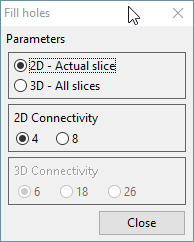
\includegraphics[scale=0.7]{mask_manual_fill_holes_window_en.png}
\caption{Dialog to configure the parameters of Fill holes manually tool.}
\label{fig:mask_manual_fill_holes_window}
\end{figure}

It is possible to fill hole on a mask slice (\textbf{2D - Actual slice}) or on all slices, selecting the option (\textbf{3D - All slices}). The connectivity may also be configured: $4$ or $8$ for 2D and $6$, $18$ and $26$ for 3D.

After configuring the desired parameters left-click on holes to fill them. Figure~\ref{fig:mask_fill_hole}.a shows a mask with some holes and other mask with the holes filled (Figure~\ref{fig:mask_fill_hole}.b). Click on the close button or close the dialog to deactivate this tool.

\begin{figure}[!htb]
  \centering
  \subfloat[Holes]{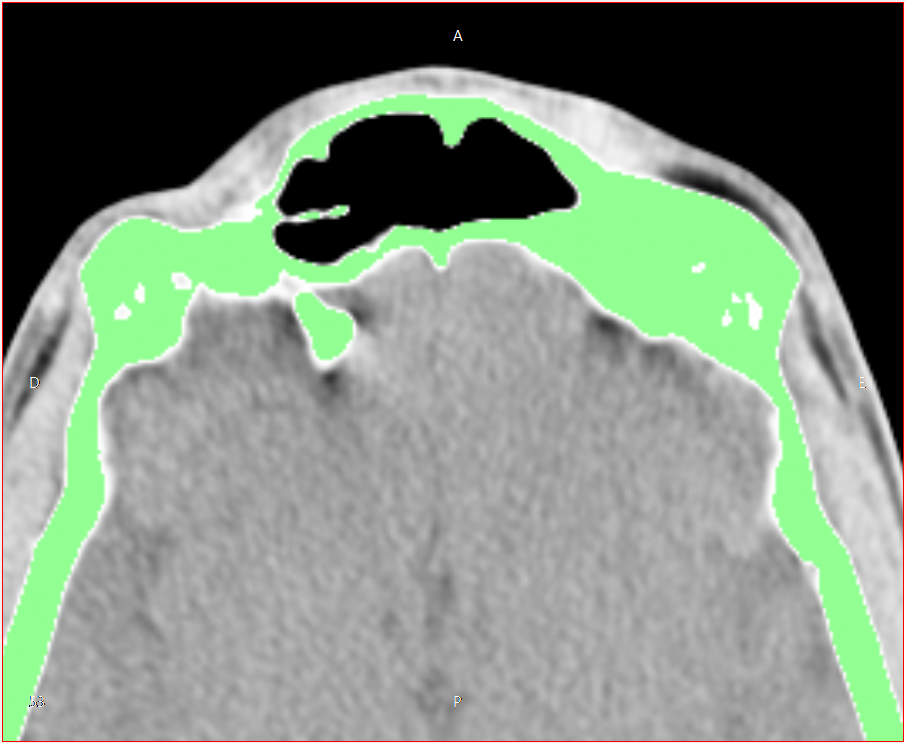
\includegraphics[width=0.4\textwidth]{mask_axial_with_hole.png}}  \qquad
  \subfloat[Holes filled]{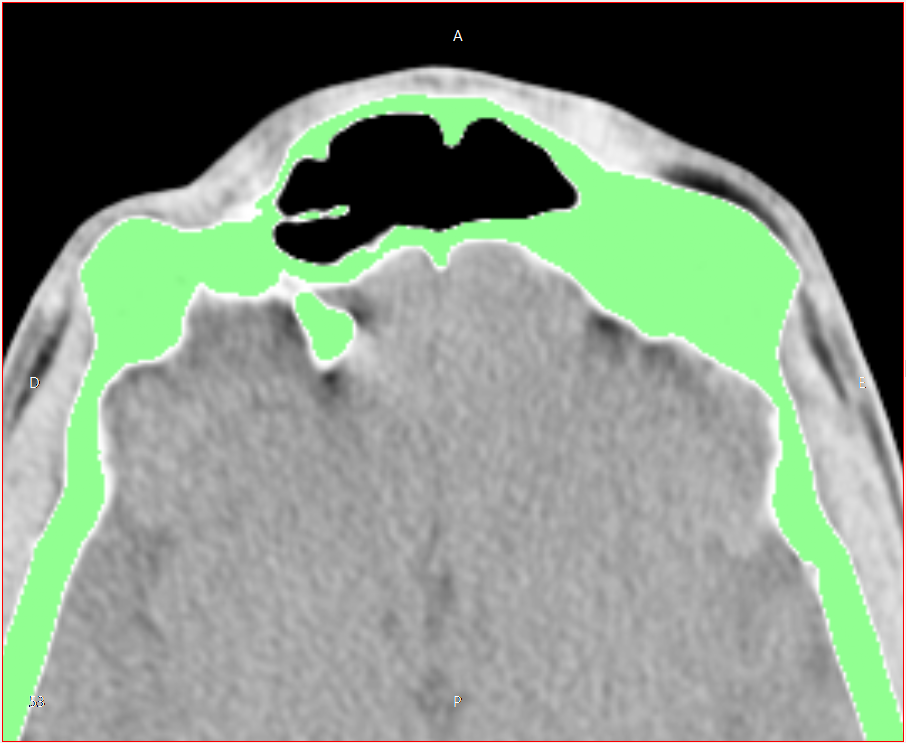
\includegraphics[width=0.4\textwidth]{mask_axial_filled_hole.png}}
  \hfill
  \caption{Example of mask with holes filled.}
  \label{fig:mask_fill_hole}
\end{figure}


\section{Fill holes automatically}

To open this tool go to the \textbf{Tools} menu, select \textbf{Mask} then \textbf{Fill holes automatically} (Figure~\ref{fig:menu_mask_automatic_fill_holes}). This will open a dialog to configure the parameters. This tool doesn’t require the user to click on holes he desire to fill. This tool will fill the holes based on the \textbf{max hole size parameter} given in number of voxels (Figure~\ref{fig:mask_automatic_fill_holes_window}).

\begin{figure}[!htb]
\centering
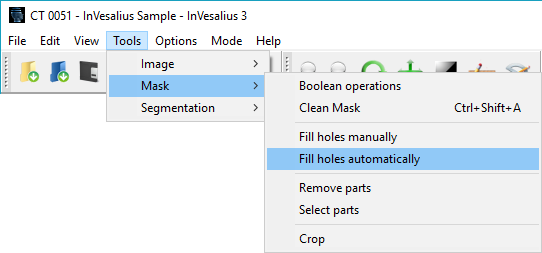
\includegraphics[scale=0.4]{menu_mask_automatic_fill_holes_en.png}
\caption{Menu to open the Fill holes automatically tool.}
\label{fig:menu_mask_automatic_fill_holes}
\end{figure}

\begin{figure}[!htb]
\centering
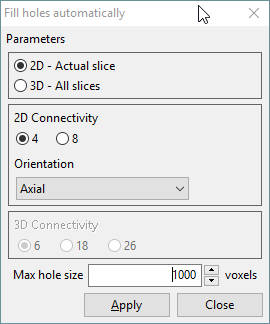
\includegraphics[scale=0.7]{mask_automatic_fill_holes_window_en.png}
\caption{Dialog to configure the parameters used to fill the holes.}
\label{fig:mask_automatic_fill_holes_window}
\end{figure}

Holes can also be filled on a mask slice (\textbf{2D - Actual slice}) or on all slices, selecting the option (\textbf{3D - All slices}. The connectivity will thus be $4$ or $8$ to 2D and $6$, $18$ and $26$ to 3D. If 2D, the user must indicate in which orientation window the holes will be filled.

After setting the parameters click \textbf{Apply}. If the result is not suitable set another hole size value or connectivity. Click \textbf{Close} to close this tool.

\section{Remove parts}

After generating a surface, it is recommended to remove the unwanted disconnected parts from a mask. This way the surface generation will use less RAM and make the process quicker. To remove any unwanted parts, go to the \textbf{Tools} menu, select \textbf{Mask} and then \textbf{Remove Parts} (Figure~\ref{fig:menu_mask_remove_part}). A dialog will be shown to configure the selection parameters  (Figure~\ref{fig:mask_remove_parts_window}).

It’s possible to select disconnected parts only on a mask slice (\textbf{2D - Actual slice}) or on all slices (\textbf{3D - All slices}); users may also configure the connectivity at the same time.

\begin{figure}[!htb]
\centering
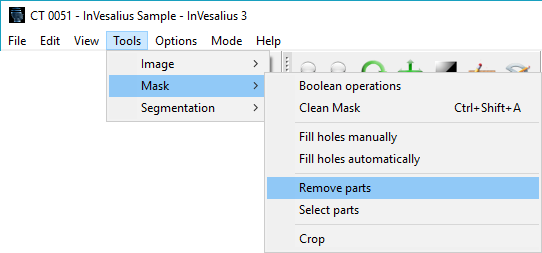
\includegraphics[scale=0.4]{menu_mask_remove_part_en.png}
\caption{Menu to open the Remove parts tool.}
\label{fig:menu_mask_remove_part}
\end{figure}

\begin{figure}[!htb]
\centering
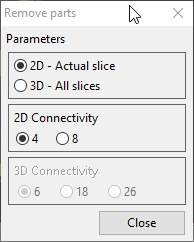
\includegraphics[scale=0.7]{mask_remove_parts_window_en.png}
\caption{Dialog to configure the parameters used in Remove parts.}
\label{fig:mask_remove_parts_window}
\end{figure}

After selecting the desired parameters click with the \textbf{left-button} of the mouse on the region you want to remove. Figure~\ref{fig:mask_removed_part} shows an example of a mask before and after the removal of unused parts. Click \textbf{Close} to stop using this tool.

\begin{figure}[!htb]
  \centering
  \subfloat[Input image]{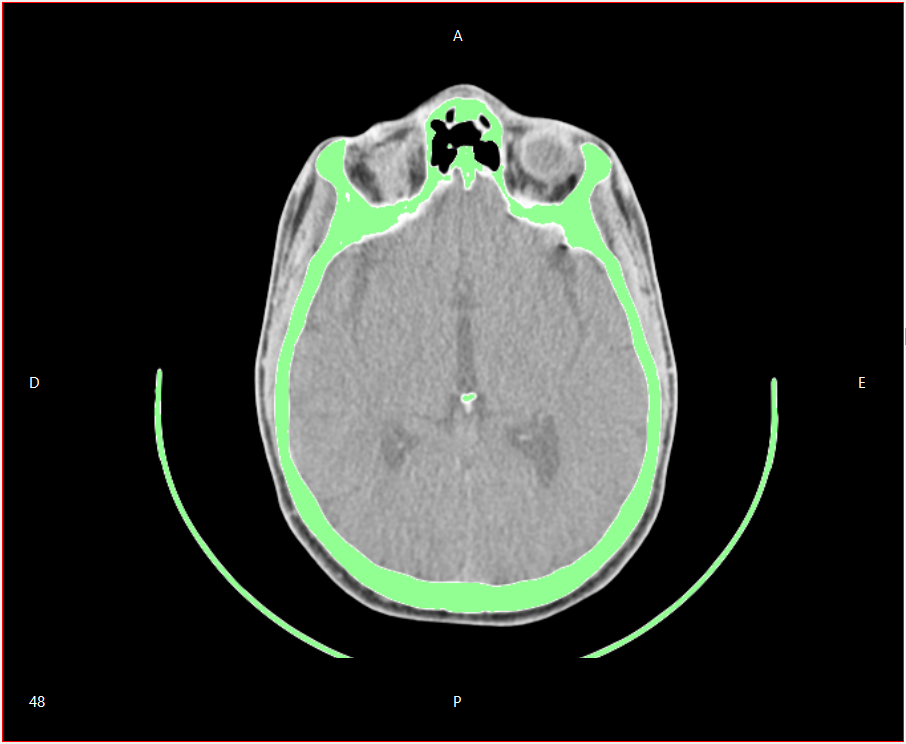
\includegraphics[width=0.45\textwidth]{mask_axial_complete.png}}  \qquad
  \subfloat[Remove the tomograph support]{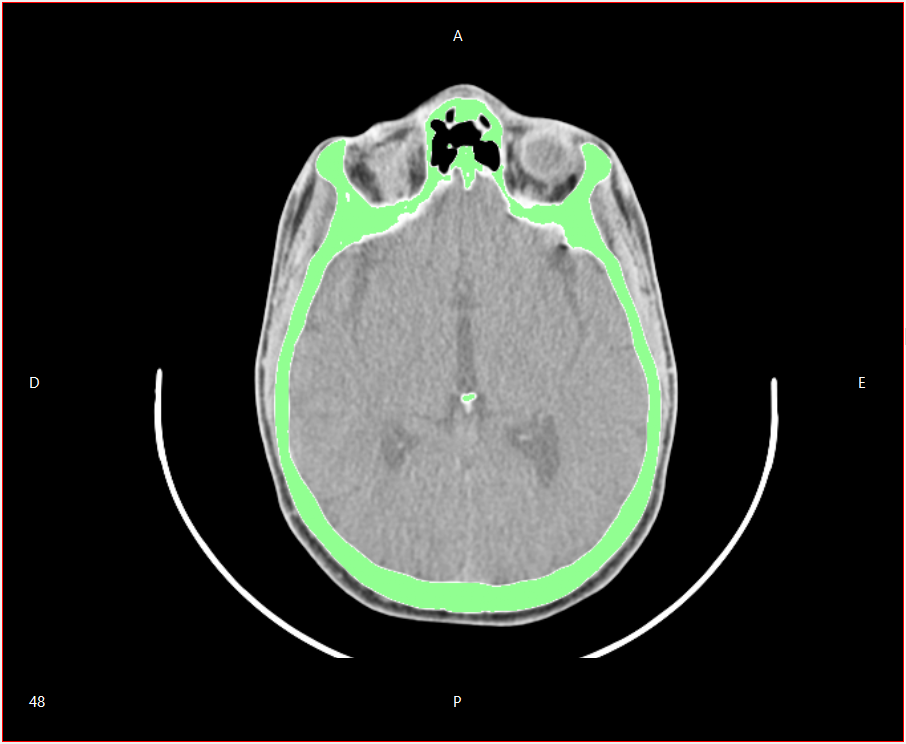
\includegraphics[width=0.45\textwidth]{mask_axial_selected_part.png}}
  \hfill
  \caption{Example of region remove from a mask.}
  \label{fig:mask_removed_part}
\end{figure}

\section{Select parts}

To open the Select parts tool, access the \textbf{Tools} menu, select \textbf{Mask} then \textbf{Select parts} (Figure~\ref{fig:menu_mask_select_part}). A dialog will be shown to configure the the name of the new mask and the connectivity ($6$, $18$ or $26$).

To select a region, \textbf{left-click} on a pixel; multiple regions can be selected. The selected region(s) will be shown with a red mask. After selecting all the wanted regions, click \textbf{OK} to create a new mask with the selected regions. Figure~\ref{fig:mask_selected_part}.a shows a region selected in red. Figure~\ref{fig:mask_selected_part}.b shows the selected region in a new mask.

\begin{figure}[!htb]
\centering
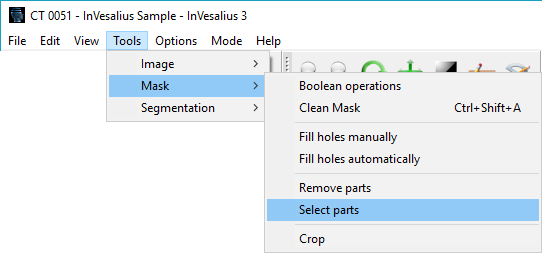
\includegraphics[scale=0.4]{menu_mask_select_part_en.png}
\caption{Menu to open the Select parts tool.}
\label{fig:menu_mask_select_part}
\end{figure}

\begin{figure}[!htb]
\centering
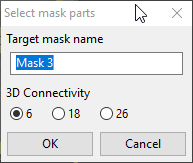
\includegraphics[scale=0.7]{mask_select_part_en.png}
\caption{Dialog to configure the parameters of Select parts tool.}
\label{fig:mask_select_part}
\end{figure}

\begin{figure}[!htb]
  \centering
  \subfloat[Region selected in red]{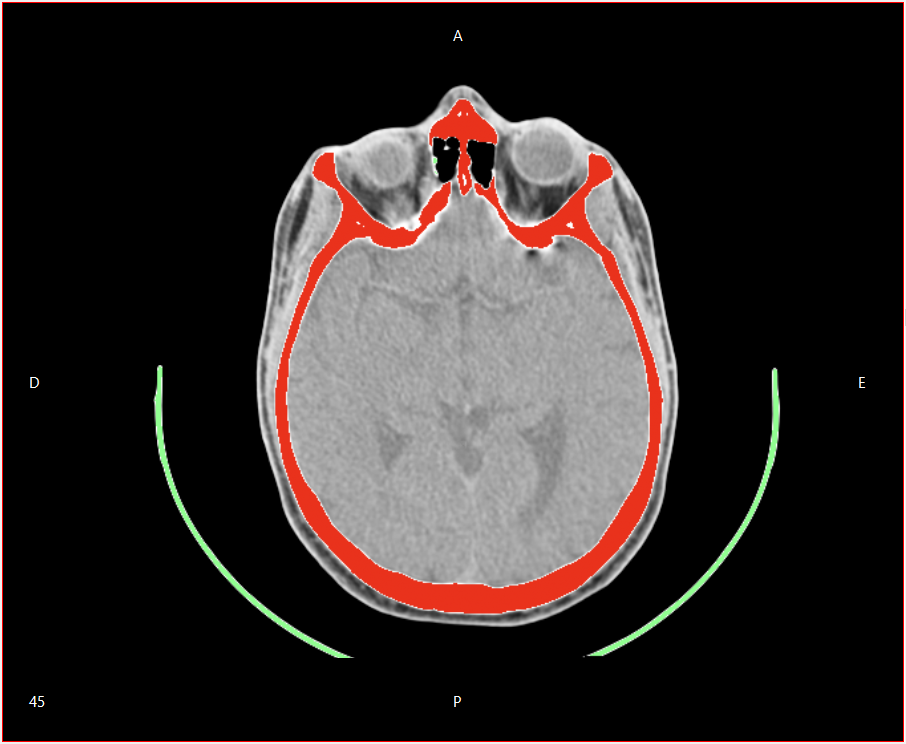
\includegraphics[width=0.45\textwidth]{mask_axial_select_part_pt.png}}  \qquad
  \subfloat[Final image with only the selected region]{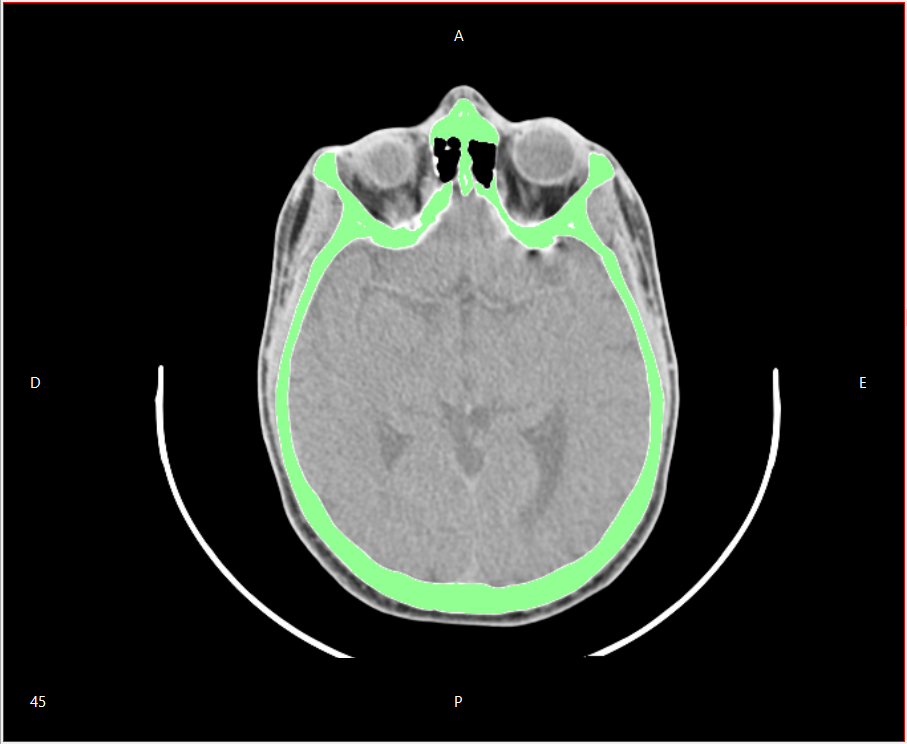
\includegraphics[width=0.45\textwidth]{mask_axial_selected_part_pt.png}}
  \hfill
  \caption{Example of mask region selection.}
  \label{fig:mask_selected_part}
\end{figure}

\section{Crop}

The crop tool allows users to select and use a specific section of image of interest. This may reduce the amount of information needed to be processed when generating a surface. To open, access the \textbf{Tool} menu, then \textbf{Mask} and \textbf{Crop} (Figure~\ref{fig:menu_mask_crop}).

\begin{figure}[!htb]
\centering
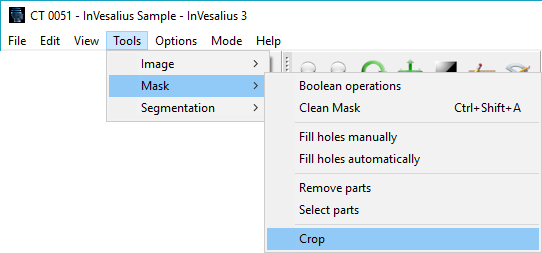
\includegraphics[scale=0.4]{menu_mask_crop_en.png}
\caption{Menu open the Crop tool.}
\label{fig:menu_mask_crop}
\end{figure}

A box allowing for the selection of a specific area will then be displayed.